% uncomment this to get the answer
%\printanswers
%\newtheorem{exercise}[theorem]{Exercise}

\documentclass[a4paper,12pt]{article}%
\usepackage{amsmath}
\usepackage{amsfonts}
\usepackage{amssymb}
\usepackage{graphicx}
\usepackage{hyperref}%
\setcounter{MaxMatrixCols}{30}
%TCIDATA{OutputFilter=latex2.dll}
%TCIDATA{Version=5.50.0.2953}
%TCIDATA{CSTFile=40 LaTeX article.cst}
%TCIDATA{Created=Tuesday, September 15, 2015 18:10:19}
%TCIDATA{LastRevised=Monday, October 11, 2021 15:30:25}
%TCIDATA{<META NAME="GraphicsSave" CONTENT="32">}
%TCIDATA{<META NAME="SaveForMode" CONTENT="1">}
%TCIDATA{BibliographyScheme=Manual}
%TCIDATA{<META NAME="DocumentShell" CONTENT="Standard LaTeX\Blank - Standard LaTeX Article">}
%BeginMSIPreambleData
\providecommand{\U}[1]{\protect\rule{.1in}{.1in}}
%EndMSIPreambleData
\newtheorem{theorem}{Theorem}
\newtheorem{acknowledgement}[theorem]{Acknowledgement}
\newtheorem{algorithm}[theorem]{Algorithm}
\newtheorem{axiom}[theorem]{Axiom}
\newtheorem{case}[theorem]{Case}
\newtheorem{claim}[theorem]{Claim}
\newtheorem{conclusion}[theorem]{Conclusion}
\newtheorem{condition}[theorem]{Condition}
\newtheorem{conjecture}[theorem]{Conjecture}
\newtheorem{corollary}[theorem]{Corollary}
\newtheorem{criterion}[theorem]{Criterion}
\newtheorem{definition}[theorem]{Definition}
\newtheorem{example}[theorem]{Example}
\newtheorem{lemma}[theorem]{Lemma}
\newtheorem{notation}[theorem]{Notation}
\newtheorem{problem}[theorem]{Problem}
\newtheorem{proposition}[theorem]{Proposition}
\newtheorem{remark}[theorem]{Remark}
\newenvironment{proof}[1][Proof]{\noindent\textbf{#1.} }{\ \rule{0.5em}{0.5em}}
\newenvironment{TEUB}[1][Proof]{\noindent\textbf{#1.} }{\ \rule{0.5em}{0.5em}}
\def\NOMDOSSIER{Bayesian Estimation of \\DSGE Models}
\def\NUMERODOSSIER{4}
\def\LECTURENAME{Bayesian Techniques \\ in Macroeconomics}
\def\DIPLOMA{Master - Quantitative Economics, 2$^{nd}$ year}
\def\UNIV{Paris-Dauphine \& PSL Universities}
\def\WEBPAGE{\href{https://vermandel.org/btm/}{https://vermandel.org/btm}}



%\def\LECTURENAME{Bayesian Techniques \\ in Macroeconomics}
\def\DIPLOMA{Master - Quantitative Economics, 2$^{nd}$ year}
\def\UNIV{Paris-Dauphine \& PSL Universities}
\def\WEBPAGE{\href{https://vermandel.org/btm/}{https://vermandel.org/btm}}


% basic  stuff
\usepackage[T1]{fontenc}
\usepackage{lmodern}
\usepackage{graphicx}
\usepackage{color}
\usepackage{xcolor}
\usepackage{hyperref}
\usepackage{eurosym}
\usepackage{natbib}
\usepackage{minted}
\usepackage[most]{tcolorbox}
\usetikzlibrary{calc}
\definecolor{deepblue}{RGB}{0,129,188}
\definecolor{deepblue2}{RGB}{0,26,153}
\definecolor{deepgreen}{RGB}{73,155,202}
\definecolor{mygray}{gray}{0.9}
\definecolor{myblue}{RGB}{0,163,243}

\setlength\parskip{.4em plus 0.1em minus 0.2em}
\setlength{\parindent}{15pt}%

% the page size
\usepackage{geometry}
\geometry{a4paper, top=1.5cm, left=1cm, right=1.0cm, bottom=1.0cm, includehead, includefoot}
\graphicspath{{../},{../../},{/chap1},{/chap2},{/chap3},{/chap4},{/chap5},{/chap6},{../2018_macroeconometrics/}}
\pdfoptionpdfinclusionerrorlevel=0


% TOC programming
\usepackage{tocloft}
\setlength{\cftbeforesecskip}{2pt}
\setcounter{tocdepth}{1} % hide subsection in TOC

%%% BULLET LIST ITEMS
\usepackage{bm}
\newcommand{\localtextbulletone}{\textcolor{deepblue2}{\bm{$\circ$}}}
\renewcommand{\labelitemi}{\localtextbulletone}

% section programming 
\usepackage[calcwidth]{titlesec}
\titleformat{\section}% sectioning command formatted
            {\bfseries\LARGE\color{deepblue2}}% font commands applied to whole
            {\thesection .}% label
            {0.5em}% separation between label and title
            {}% commands before section title
            [{\titlerule[1pt]}]% commands after

\titleformat{\part}% sectioning command formatted
            {\bfseries\large}% font commands applied to whole
            {PARTIE \thepart ~:}% label
            {0.5em}% separation between label and title
            {}% commands before section title
            [{\titlerule[1pt]}]% commands after
			
%\renewcommand{\questionshook}{%
%   \setlength{\labelsep}{6pt}%  --> espace entre la puce et le début du texte
%    \setlength{\leftmargin}{0pt}%  --> espace entre le texte et la marge gauche (sauf pour la premiere ligne)
%    \setlength{\labelwidth}{30pt}% --> taille de la boite contenant la puce. Aligné à droite. Si taille < taille de la puce, la taille de la boite est egale à la taille de la puce
%   \setlength{\listparindent}{\parindent}% --> indentation des paragraphe dans la liste
%    \setlength{\itemindent}{30pt}% --> espace entre la marge et la puce
    %\setlength{\itemsep}{0pt}% --> espace entre les items (auquel s'ajoute \parsep}
%}
%\renewcommand\thequestion{\arabic{question}}
%\renewcommand{\questionlabel}{Question No.~\thequestion.}

%Pdf HYPPERREF STUFF
\hypersetup{
colorlinks=false,
	breaklinks=true,
	plainpages=false,
	%pdftitle={\letitre},
	pdfauthor={University of Paris-Dauphine},
	pdfsubject={},
	pdfcreator={TeX et TXC},
	%pdfstartpage={1},
	%pdfpagemode={FullScreen}
	pdfkeywords={DSGE, Business Cycles},
	pdfborder={0 0 0},
	bookmarksnumbered=true,
	pdfproducer={University Paris-Dauphine},     
	pdfnewwindow=true,          
	colorlinks=true,           
	linkcolor=deepblue,              
	citecolor=deepblue,            
	filecolor=black,          
	urlcolor=deepblue2 
}

% DEALING WITH BOXES
\usepackage{tcolorbox}
\newtcolorbox{mybox}[1]{colback=black!5,colframe=black!40,fonttitle=\bfseries,title=#1,fontlower=\sfdefault}
\newtcolorbox{myconsole}[1]{colback=deepblue!5,colframe=deepblue!40,fonttitle=\bfseries,title=#1,fontlower=\sfdefault}
\newtcolorbox{myresult}[1]{colback=black!5,colframe=deepgreen,fonttitle=\bfseries,title=#1,fontlower=\sfdefault}


%%% EXERCISE BOX
\newtcolorbox[auto counter]{assignment}{
  breakable,
  fonttitle=\bfseries,
  title={Assignment \thetcbcounter}
}
\newtcolorbox[auto counter]{myexercise}[1]{
  skin=enhanced,
  breakable,
  colback=white,
  colframe=gray!30,
  coltitle=black,
  fonttitle=\bfseries,
  leftrule=0.5cm,
  arc=0pt,
  outer arc=0pt,
  title={Exercise \thetcbcounter : #1}
}
\newtcolorbox{definitioniii}[1]{
  skin=enhanced,
  breakable,
  fonttitle=\bfseries,
  colback=white,
  arc=0pt,
  outer arc=0pt,
  title={#1},
  shadow={1mm}{-1mm}{0mm}{fill=gray,opacity=0.5,sharp corners}
}

% DEALING WITH THE EXAM CLASS
%\printanswers % If you want to print answers
% \noprintanswers % If you don't want to print answers
%\addpoints % if you want to count the points
% \noaddpoints % if you don't want to count the points
% Specifies the way question are displayed:
%\qformat{\textbf{Question \thequestion}\hfill}%\quad(\thepoints)\hfill}
%\definecolor{SolutionColor}{rgb}{0.8,0.9,1} % light blue
%\shadedsolutions % defines the style of the solution environment
% \framedsolutions % defines the style of the solution environment
% Defines the title of the solution environment:
%\renewcommand{\solutiontitle}{\noindent\textbf{Solution:}\par\noindent}
%\renewcommand{\questionlabel}{\textbf{~\thequestion)} }

% Table of content
\usepackage{titlesec}
\usepackage{titletoc}
\usepackage[titletoc]{appendix}
\contentsmargin{0pt}
\renewcommand\contentspage{\color{deepblue2}p. \thecontentspage}
\dottedcontents{section}[2.3em]{}{2.3em}{5pt}
\dottedcontents{subsection}[5.5em]{}{3.2em}{5pt}
\renewcommand*\contentsname{\bfseries\color{deepblue2}Content of the Handout}

% FRONT PAGE STUFF
\usepackage{setspace}
\def\FRONTPAGE{%
\begin{picture}(0,0)\unitlength=1cm
%\put (1,0) {\includegraphics[width=7.5em]{PSL.png}}
\put (7.5,-1.4) {
\includegraphics[width=.6\textwidth]{logo-upd.png}}
\end{picture}
\begin{center}
	\color{black!70}
	\ifnum\NUMERODOSSIER<1
		\rule{19cm}{.2pt}\\ \hfill Gauthier Vermandel \textcolor{deepblue2}{\bm{$\circ$}} \textit{gauthier.vermandel@dauphine.psl.eu} \\
		\vspace{2cm}
	\else
		\rule{19cm}{.2pt}\\ \hfill Fall \the\year \\
		\textbf{\large \LECTURENAME }\\
		\vspace{0.5cm}
		\UNIV \\ \DIPLOMA \\
		\vspace{0.5cm}
		Gauthier Vermandel\footnote{Department of Economics, Paris-Dauphine University. Updated slides and codes available on my website: \WEBPAGE.} \hfill \textit{gauthier.vermandel@dauphine.psl.eu} \\
		\rule[0.25cm]{19cm}{.2pt}\\
		\vspace{1cm}
	\fi
	\color{black}
  \ifnum\NUMERODOSSIER<1
	\ifnum\NUMERODOSSIER=0
		\begin{spacing}{1.25}
			\hspace{-.2cm}\textcolor{deepblue2}{\Large\textsc{A Note on}\\\textbf{\LARGE \NOMDOSSIER }}
		\end{spacing}
	 \else
		\begin{spacing}{1.25}
			\hspace{-.2cm}\textcolor{deepblue2}{\textbf{\LARGE \NOMDOSSIER }}
		\end{spacing}	 
	\fi
  \else
	\begin{center}
		\begin{minipage}{0.5\textwidth}
				\centering \textcolor{deepblue2}{ \hspace{-.23cm}\Large \textsc{ Chapter \NUMERODOSSIER }}\\ 
				\vspace{1ex}
		\end{minipage}
		 \\ \vspace{2ex}
		\begin{minipage}{0.65\textwidth}
				\begin{center}
					 \onehalfspacing
					 \textcolor{deepblue2}{ \LARGE\textbf{\NOMDOSSIER }}
					 \doublespacing
				\end{center}
		\end{minipage}
	\end{center}
  \fi
	
	\vspace{0.5cm}
\end{center}
\vspace{0.5cm}
\ifnum\NUMERODOSSIER >-1
	\tableofcontents
\fi

}

% page headers
\ifnum\NUMERODOSSIER >-1
	\usepackage{fancyhdr} %pour modification des pieds de page
	\pagestyle{fancy} % Finally, use the "fancy" page style to implement the FancyHdr headers
	\setlength{\headheight}{14.5pt}
	\fancyhf{}
	\fancyheadoffset{0\textwidth}
	\fancyfoot[C]{\color{black!60} page \thepage}
	\renewcommand{\headrulewidth}{1pt}
	\fancyhead[L]{ \color{deepblue2}\nouppercase{\rightmark}}
\fi




\newcounter{theexercise}
\setcounter{theexercise}{1}
\newenvironment{exercise}
{	
	\vspace{1cm} 
	%\begin{center}\textcolor{black!40}{\rule{6cm}{1px}\\}\end{center} 
	\Large \color{deepblue2} \underline{Exercise \arabic{theexercise}:} 
}
{ 
	\vspace{.5cm}  
	%\begin{center}\textcolor{black!40}{\rule{6cm}{1px}\\}\end{center} 
	\stepcounter{theexercise} 
}


%%%%%%%%%%%%%%%%%%%%%%%%%%%%%%%%%%% NICE COLORBOX
\tcbset{mystyle/.style={
  breakable,
  enhanced,
  outer arc=0pt,
  arc=0pt,
  colframe=myblue,
  colback=myblue!20,
  attach boxed title to top left,
  boxed title style={
    colback=myblue,
    outer arc=0pt,
    arc=0pt,
    top=3pt,
    bottom=3pt,
    },
  fonttitle=\sffamily
  }
}

\newtcolorbox{myobjs}[1][]{
  mystyle,
  title= \large\textsc{Handout Objectives},
  attach boxed title to top center,
  colframe=deepblue,
  colback=white,
   boxed title style={
    colback=deepblue,
    outer arc=2pt,
    arc=2pt,
	top=10pt,bottom=10pt
    },
  outer arc=2pt,
  arc=2pt,
}


\newtcolorbox[auto counter]{myproof}[1][]{
  mystyle,
  colback=white,
  rightrule=0pt,
  toprule=0pt,
  title=Proof \thetcbcounter,
  overlay unbroken and first={
      \path
        let
        \p1=(title.north east),
        \p2=(frame.north east)
        in
        node[anchor=west,font=\sffamily,color=myblue,text width=\x2-\x1] 
        at (title.east) {#1};
  }
}

\newtcolorbox[auto counter]{myMATLAB}[1][]{
  mystyle,
  colframe=deepblue,
  colback=deepblue!0,
  boxed title style={
    colback=deepblue
    },
  title=MATLAB box~\thetcbcounter,
  overlay unbroken and first={
      \path
        let
        \p1=(title.north east),
        \p2=(frame.north east)
        in
        node[anchor=west,font=\sffamily,color=deepblue,text width=\x2-\x1] 
        at (title.east) {#1};
  }
}

\newcommand{\MATLABbox}[1]{
	\vspace{2ex}
	\begin{myMATLAB}[\detokenize{#1}.m]
	%\inputminted[bgcolor=black!10, frame=lines, framesep=8\fboxrule, rulecolor=\color{black!30},framerule=1pt, linenos=true,numbersep=3pt,fontsize=\footnotesize]{matlab}{codes/\detokenize{#1}.m}
	{\centering\includegraphics[width=\textwidth,trim={1cm 0 1cm 0},clip]{codes/\detokenize{#1}.png}}
	\end{myMATLAB}
	\vspace{2ex}
}

\newcommand{\MATLABboxPDF}[1]{
	\vspace{2ex}
	\begin{myMATLAB}[\detokenize{#1}.m]
	%\inputminted[bgcolor=black!10, frame=lines, framesep=8\fboxrule, rulecolor=\color{black!30},framerule=1pt, linenos=true,numbersep=3pt,fontsize=\footnotesize]{matlab}{codes/\detokenize{#1}.m}
	{\centering\includegraphics[width=\textwidth,trim={1cm 0 1cm 0},clip]{codes/\detokenize{#1}.pdf}}
	\end{myMATLAB}
	\vspace{2ex}
}


\newcommand{\MATLABboxNoFig}[1]{
	\vspace{2ex}
	\begin{myMATLAB}[\detokenize{#1}.m!]
	\inputminted[bgcolor=black!10, frame=lines, framesep=8\fboxrule, rulecolor=\color{black!30},framerule=1pt, linenos=true,numbersep=3pt,fontsize=\footnotesize]{matlab}{codes/\detokenize{#1}.m}
	%{\centering\includegraphics[width=\textwidth]{codes/#1.png}}
	\end{myMATLAB}
	\vspace{2ex}
}

%%%% MAKE CODE IN BLUE PLZ
\let\oldtextsf\textsf
\renewcommand{\textsf}[1]{\textcolor{deepblue}{\oldtextsf{#1}}}

\begin{document}
\FRONTPAGE%

%TCIMACRO{\TeXButton{BeginDefinition}{\vspace{4ex}
%\begin{myobjs}}}%
%BeginExpansion
\vspace{4ex}
\begin{myobjs}%
%EndExpansion


\begin{itemize}
\item Estimating a DSGE model with Bayesian techniques;

\item Decomposing business-cycle fluctuations into multiple exogenous disturbances;

\item Producing forecasts and diagnostic checks.
\end{itemize}

%

%TCIMACRO{\TeXButton{EndDef}{\end{myobjs}}}%
%BeginExpansion
\end{myobjs}%
%EndExpansion


\newpage

\section{A\ Bayesian perspective}

We estimate a state-space linear model using Bayesian techniques as in
\cite{fernandez2004comparing} and \cite{smets2007shocks}. Non-calibrated
parameters are estimated using the Bayesian maximum likelihood principle (see
\cite{an2007bayesian} for an extensive presentation). As exemplified by
\cite{smets2003estimated} and \cite{smets2007shocks}, this approach can
fruitfully be applied to macroeconomic models as it allows a DSGE model to
perform as well as non-constrained VAR model in explaining macroeconomic time
series. In our estimation we follow closely each of the steps defined by
\cite{smets2003estimated}.\footnote{The successive steps of this estimation
strategy are presented by \cite{smets2003estimated} as follows:
\textquotedblleft this econometric approach attempts to provide a full
characterisation of the observed data series. For example, following
\cite{sargent1989two}, a number of authors have estimated the structural
parameters of DSGE models using classical maximum likelihood methods. These
maximum likelihood methods usually consist of four steps. In the first step,
the linear rational expectations model is solved for the reduced form state
equation in its predetermined variables. In the second step, the model is
written in its state space form. This involves augmenting the state equation
in the predetermined variables with an observation equation which links the
predetermined state variables to observable variables. In this step, the
researcher also needs to take a stand on the form of the measurement error
that enters the observation equations. The third step consists of using the
Kalman filter to form the likelihood function. In the final step, the
parameters are estimated by maximising the likelihood function. Alternatively
within this strong interpretation, a Bayesian approach can be followed by
combining the likelihood function with prior distributions for the parameters
of the model, to form the posterior density function. This posterior can then
be optimised with respect to the model parameters either directly or through
Markov Chain Monte Carlo (MCMC) sampling methods.\textquotedblright\ $\ \ $}

\subsection{Building the likelihood function}

Recall that in the first handout, any macroeconomic model with expectations
can be cast in a compact form as follows:%
\begin{equation}
\mathbb{E}_{t}\left[  f_{\Theta}\left(  x_{t+1},x_{t},x_{t-1},\epsilon
_{t}\right)  \right]  =0 \label{eq non linear system}%
\end{equation}
where $f_{\theta}$\ is the non-linear relation across variables $x_{t}$,
stochastic innovations $\epsilon_{t}$, for a given set of structural
parameters $\Theta$. By applying linearization methods

By applying linearization methods on the system of non-linear equation, it is
possible to get a solution of the form
\begin{equation}
\hat{x}_{t}=F\hat{x}_{t-1}+G\epsilon_{t}, \label{eq: non linear DR}%
\end{equation}
where elements in matrices $F$\ and $G$ are functions of structural parameters
$\Theta$.

Let $H$\ be the selection matrix of observable variables -- a subset of
$\hat{x}_{t}$ -- \ such that endogenous variables reads as $y_{t}=H\hat{x}%
_{t}+v_{t}$ with $v_{t}$ the measurement errors. Then it is possible following
the application of a filter (e.g. Kalman, inversion, particle,...) to get the
errors of prediction:%
\[
S_{t}=Y_{t}-E_{t-1}\{y_{t}\},
\]
where $E_{t-1}\{y_{t}\}$\ is an output from the statistical filter and $Y_{t}%
$\ is a sample with $n$ observed variables and $T$ periods.\ 

The errors of predictions of the estimated model follows $S_{t}\sim
\mathcal{N}(\mu_{t},\Omega_{t})$ with $\mu_{t}$\ the mean and $\Omega_{t}%
$\ the variance-covariance of errors of predictions, the general expression of
the likelihood function reads as follows:%
\begin{equation}
\log\mathcal{L}\left(  \theta|Y_{T},...Y_{1}\right)  =-\frac{nT}{2}\log
(2\pi)-\frac{1}{2}\sum_{1}^{T}\log\left(  |\Omega_{t}|\right)  -\frac{1}%
{2}\sum_{1}^{T}S_{t}^{\prime}\Omega_{t}^{-1}S_{t}.
\end{equation}


The aim is to estimate the vector of parameters $\theta,$ a subset of all the
structural parameters of a model $\theta\in\Theta$. Finally, in most
softwares, it's easier to minimize than maximize, so the maximum likelihood
estimator reads as follows:%
\begin{equation}
\hat{\theta}_{MLE}=\arg\min_{\{\theta\}}\left\{  -\log\mathcal{L}\left(
\theta|Y_{T},...Y_{1}\right)  )\right\}
\end{equation}


Note that errors of predictions $S_{t}$\ are actually a function of estimated
parameters $\theta$, i.e. some parameters values may improve the forecasting
performance of the model, and thus reduce the volatility of the errors of
predictions $\Omega_{t}$. So the idea is to pick a value of $\hat{\theta
}_{MLE}$\ that maximize the joint densities.

\subsection{Adding prior information}

The Bayesian approach consists in defining an \textit{a priori} distribution
$p(\theta)$ on the structural parameters of $\theta$ that concerns both a
prior value for this parameter and a distribution. The Bayesian estimate of a
parameter thus mixes the prior mean with the maximum likelihood estimate. The
choice of the initial values for the prior parameters requires an intuition
for their role in the economy. We follow the standard practice of the
literature in choosing one of the following probability distribution for
parameters: the Normal distribution ($\mathcal{N}$), the Beta distribution
($\mathcal{B}$, for parameters with values lying between 0 and 1), the Gamma
distribution ($\mathcal{G}$, for priors which allow relatively diffuse and
positive support) and the Inverse Gamma distribution ($\mathcal{IG}$, for
shocks, as this distribution allows us to choose priors that are strongly
diffuse and positive).

The estimates of the parameters are updated using the dataset $Y$ according to
Bayes' rule:
\begin{equation}
p(\theta|Y)=\frac{L(\theta|Y)p(\theta)}{p(Y)}\propto L(\theta|Y)p(\theta),
\end{equation}
where $L(\theta|Y)$ denotes the likelihood function, $p(\theta|Y)$ is the
posterior distribution of the parameters and $p(Y)$ is the marginal likelihood
(marginal data density).

Obtaining the analytical expression for the likelihood function is generally
not possible. However, the posterior distribution of the model parameters can
be constructed numerically by applying Markov Chain Monte Carlo (MCMC)
methods. Finally, we compute the posterior moments of the parameters using a
sufficiently large number of draws, having made sure afterwards that the MCMC
algorithm has converged.%
\begin{equation}
\hat{\theta}_{BE}=\arg\max_{\theta}L(\theta|Y)p(\theta)
\end{equation}


One main advantage of DSGE models compared to VARs concerns the evaluation of
monetary policy. DSGE models replicate time series by the responses of agents
to different sequences of shocks. Once we have estimated all the sequences of
shocks and the reaction parameters of households, firms and monetary
authorities, we can perform counterfactual analyses by changing the parameters
of monetary policy. Counterfactual scenarios can be derived from the estimated
model by optimizing the policy coefficients in the Taylor to see how well the
economy would have performed under an alternative policy regime.

\subsection{An illustration with the RBC\ filter}

\textsf{Generating artificial series.\ }Consider our 3\ equation RBC\ model
estimated with maximum likelihood and inversion filter (we could have done the
same with the Kalman filter, but it does not fit into one single MATLAB file).

Recall that in the previous handout we had done the following:

\begin{itemize}
\item Simulating a model for 200 periods, we next assumeed that only
consumption was observable, and so we used consumption to retrieve the
sequence of productivity shocks that generated the data.

\item The distribution of productivity errors is given by $\varepsilon_{t}%
\sim\mathcal{N}(0,Q)$, let us assume that we want to estimate $Q$, i.e.\ the
variance(-covariance) of errors. The true value of \underline{$Q$\ is $Q=1$}.

\item The likelihood function is given by
\[
\log L(\hat{Q}|\varepsilon_{T},...\varepsilon_{1})=-\frac{nT}{2}\log
(2\pi)-\frac{1}{2}\sum_{1}^{T}\log\left(  |\hat{Q}|\right)  -\frac{1}{2}%
\sum_{1}^{T}\varepsilon_{t}^{\prime}\hat{Q}^{-1}\varepsilon_{t}.
\]


\item The Maximum Likelihood estimation is given by the value of Q that
minimizes -$\log L$.
\end{itemize}

\textsf{Setting prior information.\ }Now we can introduce bayesian
econometrics.\ Which prior can we set for Q? The best distribution would be
one with a positive support, but for clarity purpose we pick the most simple
distribution: the Gaussian distribution. Dynare, and most of macroeconomic
papers, express any distribution into two moments: the mean and standard
deviation of the distribution.\ Since a gaussian distribution is already
expressed in term of mean/std, it's straightforward to parametrize the prior.\ 

Let us assume that the econometrician have some information about the
distribution of $Q$ and set as initial value $\hat{Q}\sim\mathcal{N}%
(1,0.10)$.\ The joint probability density of observing our data (i.e. the
log-likelihood function) is now augmented by the probability density of some
estimated parameters, that we refer to as priors, denoted $P\left(
\theta\right)  $.\ Since our prior is $\hat{Q}\sim\mathcal{N}(1,0.10)$, the
log-likelihood function now reads as follows:%

\[
\underset{\text{likelihood}}{\underbrace{\log L(\hat{Q}|\varepsilon
_{T},...\varepsilon_{1})}}+\underset{\text{priors}}{\underbrace{\log p\left(
\hat{Q},1,0.10\right)  }}%
\]
where $p\left(  .\right)  $\ is a gaussian pdf with mean $1$ and stand
deviation $0.10$. This translates into MATLAB\ as:%

%TCIMACRO{\TeXButton{Minted}{\vspace{1ex}
%\begin{minted}[bgcolor=mygray,breaklines,linenos]{matlab}
%mu_Sige = 1;
%sd_Sige = .1;
%lnprior = @(x)  log(normpdf(x,mu_Sige,sd_Sige));
%\end{minted}
%\vspace{1ex}}}%
%BeginExpansion
\vspace{1ex}
\begin{minted}[bgcolor=mygray,breaklines,linenos]{matlab}
mu_Sige = 1;
sd_Sige = .1;
lnprior = @(x)  log(normpdf(x,mu_Sige,sd_Sige));
\end{minted}
\vspace{1ex}%
%EndExpansion


Let us now explore the topology of the prior function in
\autoref{fig prior pdf}.\ We can see that $p\left(  \hat{Q},1,0.10\right)
$\ is higher when $\hat{Q}$ get closer to prior mean 1, so the prior
information curbs the likelihood function in order to take some knowledge from
the econometrician about the set of estimated parameters $\theta$.

\begin{figure}[h]
\begin{center}

\includegraphics[width=.75\textwidth]{chap4/codes/priors_pdf.pdf}
\end{center}
\caption{Prior distributions of variance covariance Q}%
\label{fig prior pdf}%
\end{figure}

\textsf{Optimizing the posterior density.}\ Like for maximum likelihood, we
must optimize an objective function.\ Now this objective function is the
posterior density: the latter is proportional to the product of the prior
density and the density of the sample (i.e. the likelihood function). This
posterior distribution takes into account both the contribution of the data
(i.e.\ the log-likelihood) and the prior information.\ We solve numerically
the following minization problem to obtain the mode of posterior
distribution:
\begin{equation}
\hat{Q}_{BE}^{\text{mode}}=\arg\min_{Q}-\log L(Q|Y)-\log p(Q)
\end{equation}
%

%TCIMACRO{\TeXButton{Minted}{\vspace{1ex}
%\begin{minted}[bgcolor=mygray,breaklines,linenos]{matlab}
%theta0 = [0.01];
%theta_MLE = fmincon(@(x) -llk(x),theta0);
%theta_BE = fmincon(@(x) -(llk(x) + lnprior(x)),theta0);
%disp('Mode:')
%disp(['MLE: Est. sqrt(Q) ' num2str(sqrt(theta_MLE))])
%disp(['BE : Est. sqrt(Q) ' num2str(sqrt(theta_BE))])
%\end{minted}
%\vspace{1ex}}}%
%BeginExpansion
\vspace{1ex}
\begin{minted}[bgcolor=mygray,breaklines,linenos]{matlab}
theta0 = [0.01];
theta_MLE = fmincon(@(x) -llk(x),theta0);
theta_BE = fmincon(@(x) -(llk(x) + lnprior(x)),theta0);
disp('Mode:')
disp(['MLE: Est. sqrt(Q) ' num2str(sqrt(theta_MLE))])
disp(['BE : Est. sqrt(Q) ' num2str(sqrt(theta_BE))])
\end{minted}
\vspace{1ex}%
%EndExpansion


We call 'mode' of the distribution because it is highest local value of the
posterior density.\ We have the highest value of the posterior density, we
also need the mean of the density as well as the dispersion of the
density.\ Problem: there is no closed-form expression to draw the density of
the posterior distribution of Q. So we must use numerical techniques also
needed to evaluate the posterior.\ Economists typically use Markov Chain Monte
Carlo (MCMC) methods -- in particular the Metropolis-Hasting algorithm -- at
this purpose.

\textsf{Drawing the uncertainty through Monte Carlo methods}.The main purpose
of MH\ algorithm is to explore the parameter's space of Q by weighting the
outcomes appropriately. A Markov chain is a stochastic model describing a
sequence of possible events in which the probability of each event depends
only on the state attained in the previous event.

\begin{enumerate}
\item \textbf{Get covariance of estimated parameters.} We first need the
variance-covariance-matrix of $\theta$ with respect to the posterior
density.\ There are different ways to obtain it. In this example, we obtain it
from the inverse of the Hessian matrix as in Dynare:
\begin{equation}
\Sigma_{\theta}=\left(  \frac{\partial\left[  \log L(\theta|Y)+\log
p(\theta)\right]  }{\partial\theta}\right)  ^{-1},
\end{equation}


\item \textbf{Markov Chain initialization.}\ We initialize each Markov Chain
by setting the first starting candidate of the chain to the estimated
posterior mode $\theta_{0}^{cand}=$.$\hat{\theta}_{BE}^{\text{mode}}$. Next,
we are looking forward to exploring $i=\{1,...N\}$ different random draws of
that lies in the neighborhood of $\hat{\theta}_{BE}^{\text{mode}}$.

\item \textbf{Draw a new candidate.} We next draw for each $i=\{1,...N\}$ a
new candidate $\theta_{i}^{cand}$ based on a random gaussian perturbation of
variance $c\times\Sigma_{\theta}$:\
\begin{equation}
\theta_{i}^{cand}\symbol{126}\mathcal{N}(\theta_{i-1}^{cand},c\times
\Sigma_{\theta})
\end{equation}


Note that $c$\ is a scale parameter.\ It critically determines how large is
the exploration space.\ If c is \textquotedblleft too\textquotedblright%
\ small, the explored parameter space will be too narrow in the neiborhood of
$\hat{\theta}_{BE}^{\text{mode}}$. Conversely, if the variance of
perturbations is too big, the chain's candidate $\theta_{i}^{cand}$\ might get
stuck into a lower local minimum. I\ discuss how to pick a not
\textquotedblleft too-big-too-small\textquotedblright\ $c$ value, based a
criterion called the acceptance rate that I\ discuss hereafter.

\item \textbf{Compute the acceptance probability of the candidate.}\ Is this
new candidate $\theta_{i}^{cand}$ more favored by the data than the previous
candidate $\theta_{i-i}^{cand}$? We can compute the acceptance rate as
follows:
\begin{equation}
\alpha_{i}=\min\left(  \frac{L(\theta_{i}^{cand}|Y)\times p(\theta_{i}%
^{cand})}{L(\theta_{i-1}^{cand}|Y)\times p(\theta_{i-1}^{cand})},1\right)  .
\end{equation}
Note that if $\alpha_{i}$\ is high (i.e. close but below one), then the new
candidate is favored while if $\alpha_{i}$\ is low, then the initial candidate
is favored.

\item \textbf{Accept or reject the candidate.} Note that we are not trying to
find the best value of $\theta$ (we already have it, it's the mode of the
posterior distribution), so the decision to accept or reject must also include
a noise in order to accept candidates with low probability.%
\[
\theta_{i}^{cand}=\left\{
\begin{array}
[c]{c}%
\theta_{i}^{cand}\text{ for }\mathcal{U}(0,1)<\text{ }\alpha_{i}\text{
(accept)}\\
\theta_{i-1}^{cand}\text{ \ \ \ \ \ \ \ \ \ \ \ \ \ (reject otherwise)}%
\end{array}
\right.
\]
Note that it is thus possible to accept a candidate with a low acceptance
probability $\alpha_{i}$, however, most likely candidates will emerge as the
number of draws $i$ increases.

\item \textbf{Repeat N\ times step 3, 4 and 5.}

\item \textbf{Truncate initial values.}\ Truncate a fraction of the first
draws (to start to the $n^{th}$ draw) to make sure the chain does not depend
on the initial value $\theta_{0}^{cand}$. The Markov chain now reads as
$\{\theta_{i}^{cand}\}_{i=n}^{N}$.

\item \textbf{Analysis.}\ Analyse the posterior distribution based the
histogram of $\{\theta_{i}^{cand}\}_{i=n}^{N}$. Compare the prior with its
posterior distribution.\ Check also that the average acceptance rate,
$E(\alpha_{i})_{i=n}^{N}$, lies between 20\% to 35\%:

\begin{enumerate}
\item if $E(\alpha_{i})_{i=n}^{N}<0.2$, the explored parameter space is too
narrow and does feature the true uncertainty stemming from the data. In that
case, all the parameters will appear (erroneously) well identified identified.

\item if $E(\alpha_{i})_{i=n}^{N}<0.35$, the explored parameter space is too
large. The posterior distributions will include parameter sets that are
rejected by the data. Some parameters may appear weakly indentified while they
are actually accurately identified.
\end{enumerate}
\end{enumerate}

%

%TCIMACRO{\TeXButton{MATLABbox}{\MATLABboxPDF{bayesianRBC}}}%
%BeginExpansion
\MATLABboxPDF{bayesianRBC}%
%EndExpansion


\newpage

\section{Bayesian estimation with Dynare}

Dynare also include a quick and easy way to estimate linear DSGE\ models with
the Kalman filter and prior information. Most of the code is going to be very
similar to maximum likelihood estimation from the previous handout.\ The only
difference lies in the specification of priors, and how from the maximization
of the posterior density, we obtain the posterior distribution.

\subsection{Priors}

When we are estimating with Bayesian techniques, we need to specify prior
distributions for each parameter to be estimated. In the estimated params
section, for each estimated parameter, we declare a distribution, and specify
parameters relevant for that distribution. The syntax for this is:

\textsf{[parameter\_name], [initial\_value(optional)],
[lower\_bound(optional)], [upper\_bound(optional)], [prior\_shape],
[prior\_mean] , [prior\_standard\_deviation], [p\_3(optional)],
[p\_4(optional)], [jscale(optional)] ;}

\begin{figure}[h]
\begin{center}

\includegraphics[width=\textwidth]{chap4/codes/priors.pdf}
\end{center}
\caption{Prior distributions}%
\label{fig smoothed shocks}%
\end{figure}

\autoref{table priors} details the distributions.\ Prior specification (in
terms of shape, mean and standard deviation) allows to give more information
about the distribution of the parameters and to avoid some regions where the
likelihood function could be flat.%

%TCIMACRO{\TeXButton{BeginTable}{\begin{table}}}%
%BeginExpansion
\begin{table}%
%EndExpansion


\begin{center}%
\begin{tabular}
[c]{llll}%
Shape & Name & Support & Example(s)\\\hline\hline
\textsf{normal\_pdf} & $\mathcal{N}\left(  \mu,\sigma\right)  $ & $\left(
-\infty,+\infty\right)  $ & Policy parameters, utility curvatures,\\
\textsf{gamma\_pdf} & $\mathcal{G}\left(  \mu,\sigma\right)  $ & $\left(
0,+\infty\right)  $ & Elasticities, utility curvatures, trends\\
\textsf{beta\_pdf} & $\mathcal{B}\left(  \mu,\sigma\right)  $ & $\left[
0,1\right]  $ & Probabilities, AR-MA\ terms, shares...\\
\textsf{inv\_gamma\_pdf} & $\mathcal{IG}_{1}\left(  \mu,\sigma\right)  $ &
$\left(  0,+\infty\right)  $ & Standard deviations\\
\textsf{uniform\_pdf} & $\mathcal{U}\left(  \mu,\sigma\right)  $ & $\left(
-\infty,+\infty\right)  $ & Same as normal distribution but with lower/upper
bounds\\
\textsf{weibull\_pdf} & $\mathcal{W}\left(  \mu,\sigma\right)  $ &
$[0,+\infty)$ & For standard deviations, in particular of measurement shocks\\
\textsf{inv\_gamma2\_pdf} & $\mathcal{IG}_{2}\left(  \mu,\sigma\right)  $ &
$\left(  0,+\infty\right)  $ & Standard deviations\\\hline\hline
\end{tabular}



\end{center}

%

%TCIMACRO{\TeXButton{TableTitle}{\caption
%{Prior distributions available in Dynare \label{table priors}}}}%
%BeginExpansion
\caption{Prior distributions available in Dynare \label{table priors}}%
%EndExpansion%
%TCIMACRO{\TeXButton{EndTable}{\end{table}}}%
%BeginExpansion
\end{table}%
%EndExpansion


To illustrate the guideline for choosing a prior, let us consider first the
AR(1) term of the productivity shock process $\rho^{A}$.\ To have a stationary
model, this parameters must be below $1$ while they must be above 0\ get a
smooth response. The beta distribution meets this requirement as it has a
support on $\left[  0,1\right]  $ and will not allow this parameter to be
above 1\ or below 0. We therefore assume $\rho^{A}\sim\mathcal{B}%
(0.5,0.2)$.\ In \textsf{estimated\_params;} block, we can add the following
prior distribution as follows:%

%TCIMACRO{\TeXButton{Minted}{\vspace{1ex}
%\begin{minted}[bgcolor=mygray,breaklines,linenos]{matlab}
%estimated_params;
%rho_A,	.8,		0,	1,		beta_pdf,		.5,	.2;
%end;
%\end{minted}
%\vspace{1ex}}}%
%BeginExpansion
\vspace{1ex}
\begin{minted}[bgcolor=mygray,breaklines,linenos]{matlab}
estimated_params;
rho_A,	.8,		0,	1,		beta_pdf,		.5,	.2;
end;
\end{minted}
\vspace{1ex}%
%EndExpansion


In the previous specification, we assume that each parameter is likely to have
a mean 0\textsf{.5}\ and a standard deviation of 0.20.\ This prior is quite
uninformative as the support of this distribution allows parameters to be
estimated near 1\ or near 0.\ Conversely, an opinionated prior with a mean of
0.90 and a standard deviation of 0.01 would allow the parameter to be estimate
very close to 0.90. Economists are free to calibrate their prior, and in turn
give or not information about the estimation of the parameter.\ For instance
here, we know that monetary policy shocks are not strongly autocorrelated, a
prior information of 0.20 with standard deviation of 0.05\ could be fairly
acceptable. Even through uninformative priors are preferred, it is possible to
set tight priors but they have to be carefully justified.

Let us consider another example.\ The estimated standard deviation of a shock
has to be positive, this constraint excludes \textit{de facto} the Normal
distribution as it has a negative support. A Beta distribution could be
motivated as we want estimated shocks to be small otherwise our first order
approximation becomes irrelevant with large shocks. However, demand and supply
shocks may have a standard deviation higher than $1$, which excludes the Beta
distribution.\ It is then possible to use a Uniform distribution, as well as a
Gamma or Inverse Gamma distributions. Here, we follow \cite{smets2007shocks}
using an Inverse Gamma distribution with a mean of 0.10 and a standard
deviation of 2 such that $\sigma^{A}\sim\mathcal{IG}(0.1,2)$. Accordingly, we
add in the Dynare file the lines which code the estimation of the shocks' volatility.%

%TCIMACRO{\TeXButton{Minted}{\vspace{1ex}
%\begin{minted}[bgcolor=mygray,breaklines,linenos]{matlab}
%stderr   e_a,	.7,	0,	inf,	inv_gamma_pdf,	.1,	2;
%\end{minted}
%\vspace{1ex}}}%
%BeginExpansion
\vspace{1ex}
\begin{minted}[bgcolor=mygray,breaklines,linenos]{matlab}
stderr   e_a,	.7,	0,	inf,	inv_gamma_pdf,	.1,	2;
\end{minted}
\vspace{1ex}%
%EndExpansion


\subsection{Estimation and posteriors}

Once the priors are written in Dynare, we have to declare which variables are
observable (and they should appear in the data file as well).\ Here, we
estimate using one time series:%

%TCIMACRO{\TeXButton{Minted}{\vspace{1ex}
%\begin{minted}[bgcolor=mygray,breaklines,linenos]{matlab}
%varobs 	y;
%\end{minted}
%\vspace{1ex}}}%
%BeginExpansion
\vspace{1ex}
\begin{minted}[bgcolor=mygray,breaklines,linenos]{matlab}
varobs 	y;
\end{minted}
\vspace{1ex}%
%EndExpansion


Finally, we declare the estimation command as we did for maximum likelihood
estimations. There are lots of options for Bayesian estimation which can go
here; it's worth seeing the Dynare Manual for an overview of these options,
and resources on Bayesian estimation for what they mean.%

%TCIMACRO{\TeXButton{Minted}{\vspace{1ex}
%\begin{minted}[bgcolor=mygray,breaklines,linenos]{matlab}
%estimation(datafile=mydata,first_obs=1,mode_compute=4,
%mh_replic=20000,mh_jscale=0.5,prefilter=1,lik_init=2,bayesian_irf,irf=30) y_obs pi_obs r_obs;
%\end{minted}
%\vspace{1ex}}}%
%BeginExpansion
\vspace{1ex}
\begin{minted}[bgcolor=mygray,breaklines,linenos]{matlab}
estimation(datafile=mydata,first_obs=1,mode_compute=4,
mh_replic=20000,mh_jscale=0.5,prefilter=1,lik_init=2,bayesian_irf,irf=30) y_obs pi_obs r_obs;
\end{minted}
\vspace{1ex}%
%EndExpansion


Here, \textsf{mh\_replic}\ denotes the number of draws sampled by
Metropolis-Hastings algorithm which aims at drawing the posterior
distributions of estimated parameters. Increasing the number of draws allows
to obtain converging chains, nonetheless it is not a sufficient condition for
convergence. For small models, the number of draws can be low (roughly here
50\ 000\ draws is fine), for large scale model, it is preferable to have a
larger number of draws to get converging chains (for instance,
\cite{smets2007shocks} draws 200 000 draws). Option \textsf{lik\_init}\ set to
2\ allows Dynare to handle non-stationnary observable variables in the fit
exercise, we know that the GDP\ is a non-stationary variable requiring a
special treatment for the estimation. Option \textsf{prefilter}\ remove the
empirical mean in the observable matrix (i.e. it demeans our
sample).\ Estimating theoretical means would require to had a trend component
in the production function, which we don't do here.\ Finally, option
\textsf{mh\_jscale}\ is a parameters which has to be adjusted in order to
obtain an acceptance ratio between 20\% and 30\% (if the final acceptance rate
is below 20\%, we have to decrease \textsf{mh\_jscale} while if it is below we
have to increase 30\%). The interval for the acceptance ratio relies on
research on bayesian statistics which I\ won't develop here.

Starting the estimation exercise, Dynare loads our data file, and starts to
find the posterior mode using csminwel algorithm using optimizations methods.
The initial value of the log-likelihood function is \textsf{540.6002}, the
algorithm employed by Dynare aims at maximising the value of the
log-likelihood function by adjusting the estimated parameters.%

%TCIMACRO{\TeXButton{BeginResults}{\vspace{3ex}
%\begin{myresult}{console response}}}%
%BeginExpansion
\vspace{3ex}
\begin{myresult}{console response}%
%EndExpansion


\textsf{Initial value of the log posterior (or likelihood): 540.6002}

\textsf{-----------------}

\textsf{f at the beginning of new iteration, -540.6001819383}

\textsf{Predicted improvement: 450.236373200}

\textsf{lambda = 1; f = -540.5959836}

\textsf{lambda = 0.33333; f = -761.5328209}

\textsf{lambda = 0.64439; f = -851.6090736}

\textsf{Norm of dx 0.30008}

\textsf{----}%

%TCIMACRO{\TeXButton{EndResults}{\end{myresult}
%\vspace{3ex}}}%
%BeginExpansion
\end{myresult}
\vspace{3ex}%
%EndExpansion


At the final iteration of the algorithm (here 58\ iterations), the improvement
performed in the last iteration is low enough for the algorithm to stop the
optimisation. The value of the log-likelihood function is now \textsf{-895.6}.
Dynare then prints in the console the mode of the posterior distribution:%

%TCIMACRO{\TeXButton{BeginResults}{\vspace{3ex}
%\begin{myresult}{console response}}}%
%BeginExpansion
\vspace{3ex}
\begin{myresult}{console response}%
%EndExpansion


\textsf{RESULTS FROM POSTERIOR ESTIMATION}

\textsf{parameters}

\textsf{ prior mean mode s.d. prior pstdev}

\textsf{rho\_A 0.500 0.9842 0.0085 beta 0.2000 }

\textsf{standard deviation of shocks}

\textsf{ prior mean mode s.d. prior pstdev}

\textsf{e\_a 0.100 1.1003 0.0454 invg 2.0000 }%

%TCIMACRO{\TeXButton{EndResults}{\end{myresult}
%\vspace{3ex}}}%
%BeginExpansion
\end{myresult}
\vspace{3ex}%
%EndExpansion


After finding the mode, the Metropolis-Hastings algorithm is employed.\ For
each chain, it samples the number of draws we specified in the estimation() command.

Here, we have two chains of 20 000 draws.\ At the end of the sampling, we will
get 40 000 samples.\ Dynare will automatically drop a certain percentages of
draws (the percentage of drops can be manually set in the estimation command).
Dynare compute the uncertainty (confidence intervals size can be manually set
in the estimation command) and the mean of each parameter using the sequence
of random samples from Metropolis-Hastings output.%

%TCIMACRO{\TeXButton{BeginResults}{\vspace{3ex}
%\begin{myresult}{console response}}}%
%BeginExpansion
\vspace{3ex}
\begin{myresult}{console response}%
%EndExpansion


\textsf{Log data density is 889.521825.}

\textsf{parameters}

\textsf{ prior mean post. mean 90\% HPD interval prior pstdev}

\textsf{rho\_A 0.500 0.9817 0.9690 0.9946 beta 0.2000}

\textsf{standard deviation of shocks}

\textsf{ prior mean post. mean 90\% HPD interval prior pstdev}

\textsf{e\_a 0.100 1.1064 1.0335 1.1844 invg 2.0000}%

%TCIMACRO{\TeXButton{EndResults}{\end{myresult}
%\vspace{3ex}}}%
%BeginExpansion
\end{myresult}
\vspace{3ex}%
%EndExpansion


Dynare prints the mean and 90\%\ confidence interval upper and lower bounds as
well as the prior standard deviation of the parameter. The posterior mean is
preferred than the mode for empirical exercises. Dynare also runs some
diagnostics to assess the convergence.

\begin{figure}[ptb]
\begin{center}
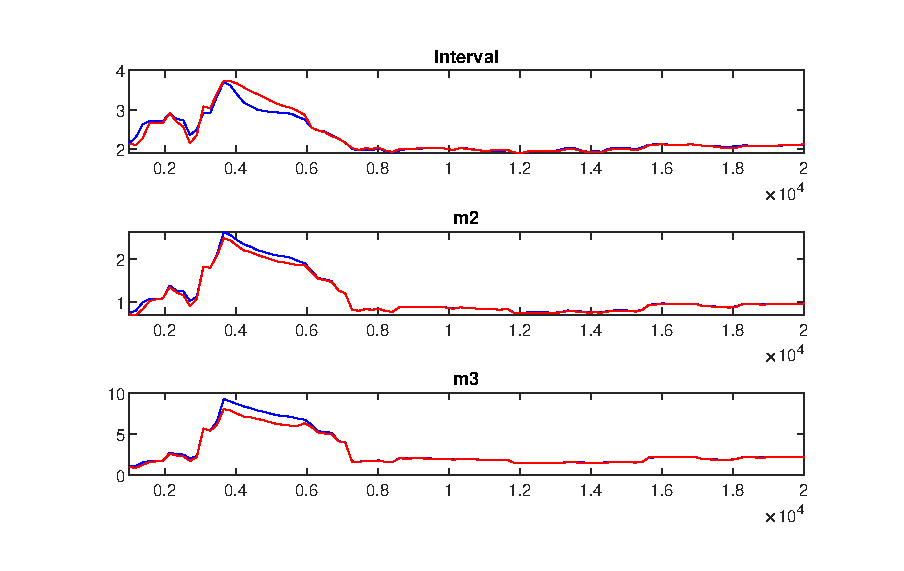
\includegraphics[
width=.5\textwidth
]{codes/diagnostics.eps}
\end{center}
\caption{Univariate convergence diagnostic, Brooks and Gelman (1998)}%
\label{fig univariate convergence}%
\end{figure}

\autoref{fig univariate convergence} reports some of the diagnostics computed
by Dynare to examine the convergence of the MCMC chains as in
\cite{brooks1998general}.\ Here for instance, the red and blue lines should
converge otherwise we should increase the number of draws, or adjust the priors/model.

\begin{figure}[ptb]
\begin{center}

\includegraphics[
width=.7\textwidth
]{chap4/codes/priorsposteriors.eps}
\end{center}
\caption{Priors (grey) and posteriors (black) distributions of estimated
parameters and mean (green).}%
\label{fig prior posterior}%
\end{figure}

\autoref{fig prior posterior} reports the prior and posterior distributions of
parameters and shocks involved in the fit exercise. It is preferable to have a
posterior distribution different than the prior one.\ Having the posterior
diverge from the prior means that your data (the likelihood in Bayes rule) is
very informative about the parameter (if the posterior distribution is not too
wide around the mode). If all your posterior estimates would coincide with the
prior mean, there would be no reason for estimation as the data does not add
any new insights. In this situation, you should calibrate rather than estimate
when the identification of your parameter is bad.

For instance in \autoref{fig prior posterior}, $\rho^{A}$ and $\sigma^{A}%
$\ are clearly well identified, \textsf{i.e.}\ data were informative for these
parameters as their priors and posteriors are different. In our situation, we
should decrease the mh acceptance rate.

%

%TCIMACRO{\TeXButton{BeginTable}{\begin{table}[h]
%\footnotesize}}%
%BeginExpansion
\begin{table}[h]
\footnotesize
%EndExpansion
%

\begin{tabular}
[c]{|l|l|}\hline
Stored in & Description\\\hline
oo\_.posterior\_mode & Parameters and shock standard errors at the posterior
mode.\\
oo\_.posterior\_std & Standard error of the estimated values at the posterior
mode.\\
oo\_.posterior\_density & Density of the posterior for each parameter (x,y
values for each parameter).\\
oo\_.prior\_density & Density of the prior for each parameter (x,y values for
each parameter).\\
oo\_.SmoothedVariables & Estimated values of each endogenous variable for all
time periods.\\
oo\_.SmoothedShocks & Estimated values of each shock for all time
periods.\\\hline
\end{tabular}
%

%TCIMACRO{\TeXButton{titre du tableau - double cliquer pour editer}%
%{\caption{Matlab's workspace after a Bayesian estimation \label
%{table workspace}}}}%
%BeginExpansion
\caption{Matlab's workspace after a Bayesian estimation \label
{table workspace}}%
%EndExpansion%
%TCIMACRO{\TeXButton{EndTable}{\end{table}
%\normalsize\newpage}}%
%BeginExpansion
\end{table}
\normalsize\newpage
%EndExpansion


\subsection{Bayesian system response}

It is also worthwhile to have a look at the bayesian system response.
\autoref{fig B IRF S} reports the system response of the model to an estimated
supply shock.\ Following a productivity shock, physical capital is more
productive, so households are more willing to postpone consumption and invest
into physical capital to get more consumption in the future. More investment
induces more demand for goods, which boost gdp both from the demand for
capital goods and by the increase in the stock of capital. The rise in income
allows the households to increase immediately consumption.\ Note that the
confidence interval is computed using Monte Carlo methods, but unlike VARs, it
does not stem from the residual uncertainty, but originates from the
parametric uncertainty. \begin{figure}[ptb]
\begin{center}

\includegraphics[
width=.7\textwidth
]{chap4/codes/birf.eps}
\end{center}
\caption{System response after an estimated supply shock}%
\label{fig B IRF S}%
\end{figure}

\subsection{Reloading results}

Obtaining the posterior distribution can take quite a lot of time, that is why
it is convenient if the model has not changed and if the posterior
distribition is acceptable, then we can reload the results from the previous
estimation as follows:%

%TCIMACRO{\TeXButton{BeginResults}{\vspace{3ex}
%\begin{myresult}{console response}}}%
%BeginExpansion
\vspace{3ex}
\begin{myresult}{console response}%
%EndExpansion


estimation(datafile=mydata,first\_obs=1,mh\_replic=0,mh\_jscale=0.5,prefilter=1,lik\_init=2,load\_mh\_file,mode\_file=NK3eq\_estim\_mode,mode\_compute=0)
y y\_obs pi\_obs r\_obs;%

%TCIMACRO{\TeXButton{EndResults}{\end{myresult}
%\vspace{3ex}}}%
%BeginExpansion
\end{myresult}
\vspace{3ex}%
%EndExpansion
%

%TCIMACRO{\TeXButton{BeginExo}{\begin{myexercise}{Fixing the estimation}
%\addcontentsline{toc}{section}{Exercise \thetcbcounter}}}%
%BeginExpansion
\begin{myexercise}{Fixing the estimation}
\addcontentsline{toc}{section}{Exercise \thetcbcounter}%
%EndExpansion


\begin{enumerate}
\item The acceptance rate is too high.\ Fix it.

\item Estimate the capital intensity parameter $\alpha$.\ Use the same prior
as \cite{smets2007shocks}.

\item Why does the steady state must be updated?
\end{enumerate}

\bigskip%
%TCIMACRO{\TeXButton{EndExo}{\end{myexercise}}}%
%BeginExpansion
\end{myexercise}%
%EndExpansion


\section{A full-fledged RBC\ model}

This model is inspired by the business cycle model of
\cite{hansen1985indivisible} which aims at fixing anomalies in the real
business cycle theory of \cite{lucas1977understanding} and
\cite{kydland1982time}. Before Hansen, the intratemporal substitution between
consumption and leisure was unable to explain large aggregate fluctuations in
hours worked/employment.

\subsection{The household}

Our economy is populated by identical and infinite living households
distributed over a continuum $j\in\left[  0,1\right]  $. The representative
household utility function reads as follows:
\[
\mathcal{U}\left(  C_{jt},H_{jt}\right)  =\frac{C_{jt}{}^{1-\sigma_{C}}%
}{1-\sigma_{C}}-\varepsilon_{t+\tau}^{H}\chi\frac{H_{jt}{}^{1+\sigma_{L}}%
}{1+\sigma_{L}}%
\]
Utility is increasing in consumption $C_{jt}$\ and decreasing in labor
$H_{jt}$ where $\sigma^{C}$ and $\sigma^{L}$\ are curvature parameters while
$\varepsilon_{t}^{H}$\ is a shock to the disutility of labor supply.
Households in this economy maximise the expected value of their utility:\
\begin{equation}
\text{$\max_{\left\{  C_{jt},H_{jt},B_{jt},K_{jt1},I_{jt}\right\}  }%
\mathbb{E}_{t}%
%TCIMACRO{\dsum \limits_{\tau=0}^{\infty}}%
%BeginExpansion
{\displaystyle\sum\limits_{\tau=0}^{\infty}}
%EndExpansion
\beta^{\tau}\mathcal{U}\left(  C_{jt},H_{jt}\right)  ,$} \label{eq hh welfare}%
\end{equation}
where $\beta$ is the discount factor. Households face an intertemporal
problem, they find the value of consumption $C_{jt}$, hours worked $H_{jt}$
and bonds $B_{jt}$\ which delivers the highest value of utility.\ They face
the following budget constraint which binds every period:%
\begin{equation}
w_{t}H_{jt}+z_{t}K_{jt-1}+r_{t-1}B_{jt-1}=C_{jt}+I_{jt}+S\left(
I_{jt},I_{jt-1}\right)  +B_{jt}+T_{jt}, \label{eq hh balance constraint}%
\end{equation}
where $w_{t}$\ is the real wage, $z_{t}$\ the remuneration of capital
services, $r_{t-1}$ is the real interest rate for bonds subscribed in $t-1$
and $T_{jt}$ are slump sum taxes which aim at financing government budget.
Here, $S\left(  I_{t},I_{t-1}\right)  $ is an investment cost function, which
replicates congestion costs when firms are simulteneous investing at the same
time.\ The functional form reads as:%
\begin{equation}
S\left(  I_{jt},I_{jt-1}\right)  =\frac{\kappa}{2}\left(  \frac{I_{jt}%
}{I_{jt-1}}-1\right)  ^{2}I_{jt-1}%
\end{equation}
where $\kappa\geq0$\ is an investment cost parameter.

The law of motion of capital also bounds the household's optimization problem:
\ \
\begin{equation}
K_{jt}=\varepsilon_{t}^{I}I_{jt}+\left(  1-\delta\right)  K_{jt-1},
\label{eq hh investment}%
\end{equation}
where $K_{jt}$\ is the stock of capital bought in $t$ (the lag is explained by
the time-to-build hypothesis regarding capital setting, \textit{i.e.}%
\ physical capital requires one period to be installed), $I_{jt}$ denotes
investment in $t$\ while parameter $\delta$\ denotes the depreciation rate of
physical capital.\ The lagrangian problem is given by:
\[
\mathcal{L}_{t}=\mathbb{E}_{t}%
%TCIMACRO{\dsum \limits_{\tau=0}^{\infty}}%
%BeginExpansion
{\displaystyle\sum\limits_{\tau=0}^{\infty}}
%EndExpansion
\beta^{\tau}\left[
\begin{array}
[c]{c}%
\frac{C_{jt+\tau}^{1-\sigma_{C}}}{1-\sigma_{C}}-\varepsilon_{t+\tau}^{H}%
\chi\frac{H_{jt+\tau}{}^{1+\sigma_{L}}}{1+\sigma_{L}}\\
+\lambda_{t+\tau}^{c}\left[
\begin{array}
[c]{c}%
w_{t+\tau}H_{jt+\tau}+z_{t+\tau}K_{jt-1+\tau}+r_{t-1+\tau}B_{jt-1+\tau}\\
-C_{jt+\tau}-I_{jt+\tau}-S\left(  I_{jt+\tau},I_{jt-1+\tau}\right)
-B_{jt+\tau}-T_{jt+\tau}%
\end{array}
\right] \\
+\lambda_{t+\tau}^{k}\left[  \varepsilon_{t+\tau}^{I}I_{jt+\tau}+\left(
1-\delta\right)  K_{jt-1+\tau}-K_{jt+\tau}\right]
\end{array}
\right]
\]
where $\lambda_{t}^{c}$\ et $\lambda_{t}^{k}$\ are lagrange multipliers
associated to the\ budget constraint and the physical capital accumulation
constraint.\ The first order conditions are given by the welfare maximisation
in $C_{jt}$, $H_{jt}$, $I_{jt}$, $K_{jt}$\ and $B_{jt}$:%
\begin{align*}
\left(  \partial C_{jt}\right)   &  :\lambda_{t}^{c}=C_{jt}{}^{-\sigma_{C}}\\
\left(  \partial H_{jt}\right)   &  :\varepsilon_{t}^{H}\chi H_{jt}%
^{\sigma^{L}}=\lambda_{t}^{c}w_{t}\\
\left(  \partial B_{jt}\right)   &  :\mathbb{E}_{t}\left\{  \frac{\lambda
_{t}^{c}}{\lambda_{t+1}^{c}}\right\}  =\beta r_{t}\\
\left(  \partial I_{jt}\right)   &  :-\lambda_{t}^{c}\left(  1+S^{\prime
}\left(  I_{jt},I_{jt-1}\right)  \right)  +\beta\lambda_{t+1}^{c}S^{\prime
}\left(  I_{jt+1},I_{jt}\right)  +\varepsilon_{t}^{I}\lambda_{t}^{k}=0\\
\left(  \partial K_{jt}\right)   &  :\varepsilon_{t}^{C}\lambda_{t}^{k}%
=\beta\mathbb{E}_{t}\left\{  \varepsilon_{t+1}^{C}\left[  \overset{}{\left(
1-\delta\right)  }\lambda_{t+1}^{k}+\lambda_{t+1}^{c}Z_{t+1}\right]  \right\}
\end{align*}
Substituting the lagrange multipliers, our optimal conditions boils down to an
Euler equation:
\begin{equation}
\beta r_{t}=\mathbb{E}_{t}\left\{  \left(  \frac{C_{jt+1}}{C_{jt}}\right)
^{\sigma_{C}}\right\}  , \label{eq household Euler}%
\end{equation}
an hour supply equation:%
\begin{equation}
W_{t}=\varepsilon_{t}^{H}\chi H_{jt}{}^{\sigma_{L}}C_{jt}{}^{\sigma_{C}}
\label{eq household labor supply}%
\end{equation}
It is possible to derive from the standard RBC\ model the endogenous asset
price denoted $q_{t}=\lambda_{t}^{k}/\lambda_{t}^{c}$, defined as the ratio
between the marginal cost of raising new capitals (Lagrangian multiplier on
capital accumulation constraint $\lambda_{t}^{k}$)\ and the marginal utility
of consumption (Lagrangian multiplier on budget constraint $\lambda_{t}^{c}$).
Variable $q_{t}$\ also refers to the well known Tobin's Q published in
\cite{tobin1969general}.\ Tobin's Q is the ratio between a physical asset's
market value and its replacement value, this ratio has considerable
macroeconomic implications as it constitutes the standard bridge between
financial markets and markets for goods and services. In steady state, the
ratio must be normalised to one to be consistent with asset pricing theory,
such that $\bar{q}=1$.

From its definition, we can thus substitute $\lambda_{t}^{k}=\lambda_{t}%
^{c}q_{t}$ in the two remaining first order conditions:%
\begin{align}
0  &  =-\lambda_{t}^{c}\left(  1+S^{\prime}\left(  I_{jt},I_{jt-1}\right)
\right)  +\beta\lambda_{t+1}^{c}S^{\prime}\left(  I_{jt+1},I_{jt}\right)
+\varepsilon_{t}^{I}\lambda_{t}^{c}q_{t}=0\label{FOC 3}\\
\varepsilon_{t}^{I}q_{t}  &  =\left(  1+S^{\prime}\left(  I_{jt}%
,I_{jt-1}\right)  \right)  -\beta\frac{\lambda_{t+1}^{c}}{\lambda_{t}^{c}%
}S^{\prime}\left(  I_{jt+1},I_{jt}\right) \\
\varepsilon_{t}^{I}q_{t}  &  =1+\kappa\left(  \frac{I_{jt}}{I_{jt-1}%
}-1\right)  I_{jt-1}+\frac{1}{r_{t}}\frac{\kappa}{2}\left(  \left(
\frac{I_{jt+1}}{I_{jt}}\right)  ^{2}-1\right)
\end{align}
It is straight forward to see that $q_{t}$\ is the real shadow value of
capital goods is a non-linear function of the (expected) growth rate of
investment.\ In absence of investment costs $\kappa=0$ (and of the investment
shock), the real value of physical capital goods becomes one.

While the first order condition on physical capital reads as:%
\begin{align}
\lambda_{t}^{c}q_{t}  &  =\beta\mathbb{E}_{t}\left\{  \left[  \overset
{}{\left(  1-\delta\right)  }\lambda_{t+1}^{c}q_{t+1}+\lambda_{t+1}^{c}%
z_{t+1}\right]  \right\} \\
q_{t}  &  =\beta\mathbb{E}_{t}\left\{  \frac{\lambda_{t+1}^{c}}{\lambda
_{t}^{c}}\left[  \overset{}{\left(  1-\delta\right)  }q_{t+1}+z_{t+1}\right]
\right\} \\
q_{t}  &  =\frac{1}{r_{t}}\mathbb{E}_{t}\left\{  \left[  \overset{}{\left(
1-\delta\right)  }q_{t+1}+z_{t+1}\right]  \right\}
\end{align}
This equation is the no-arbitrage condition between risk free assets (i.e. the
real interest rate) and risky assets (physical capital).\ The no-arbitrage
condition is determined by the equality between the current cost of purchasing
one additional unit of physical capital (left side) and the expected
discounted return of this unit. $1/r_{t}$\ reduces the expected return and
features the opportunity cost of risk free assets.

\subsection{Firms}

Firms are homogeneous and distributed on an unitary interval $i\in\lbrack0,1]$
and have the following production technology:
\begin{equation}
Y_{it}=\varepsilon_{t}^{A}{}K_{it-1}^{\alpha}H_{it}^{1-\alpha}{}
\label{eq firms production fctn}%
\end{equation}
where $Y_{it}$\ is the production, $K_{it-1}$ and $H_{it}$ are input factors,
i.e.\ the quantity of physical capital and hours involved in the production
process of firms. Finally, $\varepsilon_{t}^{A}$ denotes the productivity
shock process.

The optimisation problem can be expressed in two ways.\ 

The first one can be expressed as a profit maximisation problem:
\[
\max_{Y_{it},K_{it-1},H_{it}}Y_{it}-z_{t}K_{it-1}-w_{t}H_{it}+\lambda
_{t}\left[  \varepsilon_{t}^{A}K_{it-1}^{\alpha}{}H_{it}^{1-\alpha}{}%
-Y_{it}\right]
\]
where $\lambda_{t}$ denotes the lagrange multiplier on the supply constraint,
it can also interpreted as the marginal profit.

The second way can be viewed as an inputs minimisation problem:%
\[
\min_{K_{it},H_{it}}Z_{t}K_{it-1}+W_{t}H_{it}-\lambda_{t}\left[
\varepsilon_{t}^{A}K_{it-1}^{\alpha}{}H_{it}^{1-\alpha}{}-Y_{it}\right]
\]
where $\lambda_{t}$ denotes the lagrange multiplier on the supply constraint
and can also be interpreted as the marginal cost of producing an additional
unit of good.

First order conditions are:\
\begin{align*}
\left(  \partial K_{it-1}\right)   &  :z_{t}=\alpha\lambda_{t}\frac{Y_{it}%
}{K_{it-1}}\\
\left(  \partial H_{it}\right)   &  :w_{t}=\left(  1-\alpha\right)
\lambda_{t}\frac{Y_{it}}{H_{it}}\\
\left(  \partial Y_{it}\right)   &  :\lambda_{t}=1
\end{align*}
Replacing the lagrange multiplier, the two conditions which determine the
highest profits/lowest costs path are:%
\begin{align}
z_{t}  &  =\alpha\frac{Y_{it}}{K_{it-1}}\\
w_{t}  &  =\left(  1-\alpha\right)  \frac{Y_{it}}{H_{it}}%
\end{align}


\subsection{Aggregation and Equilibrium conditions}

Our economy is populated by two agents: households $j$ and firms $i$. Their
interactions, summarized by market clearing conditions for goods, labour and
physical capital markets, can be expressed as follows:%
\[
\underset{\text{aggregate supply}}{\underbrace{%
%TCIMACRO{\dint \nolimits_{0}^{1}}%
%BeginExpansion
{\displaystyle\int\nolimits_{0}^{1}}
%EndExpansion
Y_{it}\text{d}i}}=\underset{\text{aggregate consumption}}{\underbrace{%
%TCIMACRO{\dint \nolimits_{0}^{1}}%
%BeginExpansion
{\displaystyle\int\nolimits_{0}^{1}}
%EndExpansion
C_{jt}\text{d}j}}+\underset{\text{aggregate investment}}{\underbrace{%
%TCIMACRO{\dint \nolimits_{0}^{1}}%
%BeginExpansion
{\displaystyle\int\nolimits_{0}^{1}}
%EndExpansion
I_{jt}+S\left(  I_{jt},I_{jt-1}\right)  \text{d}j}}+\underset{\text{aggregate
public spending}}{\underbrace{\bar{G}\varepsilon_{t}^{G}}}%
\]
We assume output is driven exogenously by demand shocks, such that $\bar
{G}=g^{y}\bar{Y}$, where $g^{y}$ is the fixed
spending-to-GDP\ ratio.\ Variable $\varepsilon_{t}^{G}$ denotes the demand
shock which affects output.

Letting $Y_{t}$, $C_{t}$\ and $I_{t}$ denote the aggregate supply, consumption
and investment, the resource constraint boils down to:\
\begin{equation}
Y_{t}=C_{t}+I_{t}+S\left(  I_{t},I_{t-1}\right)  +g^{y}\bar{Y}\varepsilon
_{t}^{G}.
\end{equation}
The equilibrium on the labour market is:%
\begin{equation}
H_{t}=\underset{\text{labour demand}}{\underbrace{%
%TCIMACRO{\dint \nolimits_{0}^{1}}%
%BeginExpansion
{\displaystyle\int\nolimits_{0}^{1}}
%EndExpansion
H_{it}\text{d}i}}=\underset{\text{labour supply}}{\underbrace{%
%TCIMACRO{\dint \nolimits_{0}^{1}}%
%BeginExpansion
{\displaystyle\int\nolimits_{0}^{1}}
%EndExpansion
H_{jt}\text{d}j}},
\end{equation}
and for physical capital:%
\begin{equation}
K_{t}=\underset{\text{capital demand}}{\underbrace{%
%TCIMACRO{\dint \nolimits_{0}^{1}}%
%BeginExpansion
{\displaystyle\int\nolimits_{0}^{1}}
%EndExpansion
K_{it}\text{d}i}}=\underset{\text{capital supply}}{\underbrace{%
%TCIMACRO{\dint \nolimits_{0}^{1}}%
%BeginExpansion
{\displaystyle\int\nolimits_{0}^{1}}
%EndExpansion
K_{jt}\text{d}j}}.
\end{equation}


\subsection{Disturbances}

Our shock processes are characterized by four disturbances (in logs):%
\begin{align}
\log\left(  \varepsilon_{t}^{A}\right)   &  =\rho_{A}\log\left(
\varepsilon_{t-1}^{A}\right)  +\eta_{t}^{A}\text{ \ \ with}\ \eta_{t}^{A}%
\sim\mathcal{N}\left(  0,\sigma_{A}^{2}\right)  ,\\
\log\left(  \varepsilon_{t}^{G}\right)   &  =\rho_{G}\log\left(
\varepsilon_{t-1}^{G}\right)  +\eta_{t}^{G}\text{ with }\eta_{t}^{G}%
\sim\mathcal{N}\left(  0,\sigma_{G}^{2}\right)  ,\\
\log\left(  \varepsilon_{t}^{H}\right)   &  =\rho_{H}\log\left(
\varepsilon_{t-1}^{H}\right)  +\eta_{t}^{H}\text{ with }\eta_{t}^{H}%
\sim\mathcal{N}\left(  0,\sigma_{H}^{2}\right)  ,\\
\log\left(  \varepsilon_{t}^{I}\right)   &  =\rho_{I}\log\left(
\varepsilon_{t-1}^{I}\right)  +\eta_{t}^{I}\text{ with }\eta_{t}^{I}%
\sim\mathcal{N}\left(  0,\sigma_{I}^{2}\right)  .
\end{align}
where in steady state these shocks are normalized to one.

\subsection{Summary of the model}

The model is a set of 13\ equations and a set of 13\ endogenous variables
\{$r_{t}$,$C_{t}$,$H_{t}$,$Y_{t}$,$K_{t}$,$I_{t}$,$q_{t}$,$z_{t}$,$w_{t}%
$,$\varepsilon_{t}^{A}$,$\varepsilon_{t}^{G}$,$\varepsilon_{t}^{H}%
$,$\varepsilon_{t}^{I}$\}.
\begin{align*}
\beta r_{t} &  =\mathbb{E}_{t}\left\{  \left(  \frac{C_{t+1}}{C_{t}}\right)
^{\sigma_{C}}\right\}  \\
w_{t} &  =\varepsilon_{t}^{H}\chi H_{t}^{\sigma_{L}}C_{t}^{\sigma_{C}}\\
q_{t} &  =\frac{1}{r_{t}}\mathbb{E}_{t}\left\{  \left[  \overset{}{\left(
1-\delta\right)  }q_{t+1}+z_{t+1}\right]  \right\}  \\
\varepsilon_{t}^{I}q_{t} &  =1+\kappa\left(  \frac{I_{jt}}{I_{jt-1}}-1\right)
I_{jt-1}-\frac{1}{r_{t}}\frac{\kappa}{2}\left(  \left(  \frac{I_{jt+1}}%
{I_{jt}}\right)  ^{2}-1\right)  \\
K_{t} &  =\varepsilon_{t}^{I}I_{t}+\left(  1-\delta\right)  K_{t-1}\\
Y_{t} &  =\varepsilon_{t}^{A}K_{t-1}^{\alpha}{}H_{t}^{1-\alpha}{}\\
z_{t} &  =\alpha\frac{Y_{t}}{K_{t-1}}\\
w_{t} &  =\left(  1-\alpha\right)  \frac{Y_{t}}{H_{t}}\\
Y_{t} &  =C_{t}+I_{t}+S\left(  I_{t},I_{t-1}\right)  +g^{y}\bar{Y}%
\varepsilon_{t}^{G}\\
\log\left(  \varepsilon_{t}^{A}\right)   &  =\rho_{A}\log\left(
\varepsilon_{t-1}^{A}\right)  +\eta_{t}^{A}\\
\log\left(  \varepsilon_{t}^{G}\right)   &  =\rho_{G}\log\left(
\varepsilon_{t-1}^{G}\right)  +\eta_{t}^{G}\\
\log\left(  \varepsilon_{t}^{C}\right)   &  =\rho_{C}\log\left(
\varepsilon_{t-1}^{C}\right)  +\eta_{t}^{C}\\
\log\left(  \varepsilon_{t}^{I}\right)   &  =\rho_{I}\log\left(
\varepsilon_{t-1}^{I}\right)  +\eta_{t}^{I}%
\end{align*}


\subsection{Linearization}

The set of linearized equations reads as follows:%
\begin{align*}
\frac{1}{\sigma_{C}}\hat{r}_{t} &  =\mathbb{E}_{t}\left\{  \hat{c}%
_{t+1}\right\}  -\hat{c}_{t}\\
\hat{w}_{t} &  =\hat{\varepsilon}_{t}^{H}+\sigma_{L}\hat{h}_{t}+\sigma_{C}%
\hat{c}_{t}\\
\hat{q}_{t} &  =\beta\mathbb{E}_{t}\left\{  \left[  \overset{}{\left(
1-\delta\right)  }\hat{q}_{t+1}+\bar{Z}\hat{z}_{t+1}\right]  \right\}
-\hat{r}_{t}\\
\hat{\varepsilon}_{t}^{I}+\hat{q}_{t} &  =\kappa\bar{I}\left(  \hat{\imath
}_{t}-\hat{\imath}_{t-1}\right)  -\beta\kappa\left(  \hat{\imath}_{t+1}%
-\hat{\imath}_{t}\right)  \\
k_{t} &  =\delta\left(  \hat{\varepsilon}_{t}^{I}+\hat{I}_{t}\right)  +\left(
1-\delta\right)  \hat{k}_{t-1}\\
\hat{y}_{t} &  =\hat{\varepsilon}_{t}^{A}+\alpha\hat{k}_{t-1}{}+\left(
1-\alpha\right)  \hat{h}_{t}{}\\
\hat{z}_{t} &  =\hat{y}_{t}-\hat{k}_{t-1}\\
\hat{w}_{t} &  =\hat{y}_{t}-\hat{h}_{t}\\
\hat{y}_{t} &  =\frac{\bar{C}}{\bar{Y}}\hat{c}_{t}+\frac{\bar{I}}{\bar{Y}}%
\hat{\imath}_{t}+g^{y}\hat{\varepsilon}_{t}^{G}\\
\hat{\varepsilon}_{t}^{A} &  =\rho_{A}\hat{\varepsilon}_{t-1}^{A}+\eta_{t}%
^{A}\\
\hat{\varepsilon}_{t}^{G} &  =\rho_{G}\hat{\varepsilon}_{t-1}^{G}+\eta_{t}%
^{G}\\
\hat{\varepsilon}_{t}^{C} &  =\rho_{C}\hat{\varepsilon}_{t-1}^{C}+\eta_{t}%
^{C}\\
\hat{\varepsilon}_{t}^{I} &  =\rho_{I}\hat{\varepsilon}_{t-1}^{I}+\eta_{t}^{I}%
\end{align*}
It is also common to estimate DSGE\ models on observable taken in growth
rates.\ Therefore, letting $\Delta Y_{t}$ denote the growth rate of output,
the corresponding measurement equation reads as follows:%
\begin{align*}
\Delta Y_{t} &  =\log(Y_{t}/Y_{t-1})\\
&  =\log(Y_{t})-\log(Y_{t-1})+\log(\bar{Y}/\bar{Y})\\
&  =\log(Y_{t}/\bar{Y})-\log(Y_{t-1}/\bar{Y})\\
&  \simeq\hat{y}_{t}-\hat{y}_{t-1}%
\end{align*}
We estimate this model using output as an observable variable.

\newpage%

%TCIMACRO{\TeXButton{BeginExo}{\begin{myexercise}{Estimating the RBC model}
%\addcontentsline{toc}{section}{Exercise \thetcbcounter}}}%
%BeginExpansion
\begin{myexercise}{Estimating the RBC model}
\addcontentsline{toc}{section}{Exercise \thetcbcounter}%
%EndExpansion


Consider the code\ \textsf{fullRBC.mod} of the full-fledged RBC\ model.

\begin{enumerate}
\item Let us first include investment as an observable variable:

\begin{enumerate}
\item Add a measurement equation in the model's code for the growth of
investment $di_{t}.$

\item Add a steady state for this variable.

\item Add this observable to the \textsf{varobs}.

\item We need to include another shock in the estimation. Which one should be
pick up?\ Usually, we should include the shock that is more likely to generate
fluctuations on this variable.\ Here, the investment shock is very likely to
provide strong fluctuations on investment, so we are going to include
$\rho_{i}$\ and sd$\left(  \eta_{it}\right)  $ as parameters to estimate.

\item Run the estimation.

\item Investment adjustment cost $\kappa$ may be estimated.\ Use the priors of
\cite{smets2007shocks}
\end{enumerate}

\item Examine the historical decomposition of shock for the observable variables.

\item Examine the forecasting error decomposition.

\item Let us know include consumption as observable.\ Same as for investment,
include $dc_{t}$ in the model's block, steady state, and set it in
\textsf{varobs}. Use the government spending shock to estimate this series.

\item Finally, let us now include hours worked.\ 

\begin{enumerate}
\item This variable has no trend, so we don't need to apply the first
difference filter.\ So we need to make our equations in Dynare consistent with
the transformation of the data.\ Since data are demeaned, the data is just the
demeaned fraction of time per day devoted to work (the remaining part is the
leisure). Include a new observable:%
\[
dh_{t}=h_{t}-\bar{h}%
\]


\item Add the steady state of this variable.

\item Add this variable to the observable block.

\item Then estimate the remaining shock on the labor supply.
\end{enumerate}

\item Some other structural parameters such as $\sigma_{C}$ and $\sigma_{L}$
may be estimated.\ Use the priors of \cite{smets2007shocks}.
\end{enumerate}

%

%TCIMACRO{\TeXButton{EndExo}{\end{myexercise}}}%
%BeginExpansion
\end{myexercise}%
%EndExpansion
%

%TCIMACRO{\TeXButton{BeginExo}{\begin{myexercise}{External habits}
%\addcontentsline{toc}{section}{Exercise \thetcbcounter}}}%
%BeginExpansion
\begin{myexercise}{External habits}
\addcontentsline{toc}{section}{Exercise \thetcbcounter}%
%EndExpansion


Let us assume external consumption habits:%
\[
U\left(  C_{jt}-hC_{t-1},H_{jt+\tau}\right)  \frac{\left(  C_{jt}%
-hC_{t-1}\right)  ^{1-\sigma_{C}}}{1-\sigma_{C}}-\varepsilon_{t+\tau}^{H}%
\chi\frac{H_{jt+\tau}{}^{1+\sigma_{L}}}{1+\sigma_{L}}%
\]
Note that $C_{t-1}$\ is the previous average consumption in the population,
while $C_{t-1}$\ is agent specific.\ Habit Formation is based on catching up
with the Joneses.

The following first order conditions are affected:%
\begin{align*}
\left(  \partial C_{jt}\right)   &  :\lambda_{t}^{c}=U_{c,t}^{\prime}\\
\left(  \partial H_{jt}\right)   &  :\varepsilon_{t}^{H}\chi H_{jt}%
^{\sigma^{L}}=\lambda_{t}^{c}w_{t}\\
\left(  \partial B_{jt}\right)   &  :\mathbb{E}_{t}\left\{  \frac{\lambda
_{t}^{c}}{\lambda_{t+1}^{c}}\right\}  =\beta r_{t}%
\end{align*}


\begin{enumerate}
\item Update the first order conditions.

\item Find the steady state.

\item Linearize the equations.

\item Update the dynare files.
\end{enumerate}%

%TCIMACRO{\TeXButton{EndExo}{\end{myexercise}}}%
%BeginExpansion
\end{myexercise}%
%EndExpansion
%

%TCIMACRO{\TeXButton{small}{\footnotesize}}%
%BeginExpansion
\footnotesize
%EndExpansion
\bibliographystyle{plainnat}
\bibliography{dataref}%
%TCIMACRO{\TeXButton{small}{\normalsize}}%
%BeginExpansion
\normalsize
%EndExpansion



\end{document}
